
\subsection*{1.}

\begin{center}
\begin{tikzpicture}[thick, scale=1.5]
\node (P_-1_0) at (-2,-1.5) {$\phantom{A}$};
\node (P_0_0) at (0,-0.5) {$U$};
\draw (P_-1_0) -- (P_0_0) node[midway, above] {$\dfrac13$};
\node (P_1_0) at (2,-0) {$B$};
\draw (P_0_0) -- (P_1_0) node[midway, above] {$0{,}4$};
\node (P_1_1) at (2,-1) {$R$};
\draw (P_0_0) -- (P_1_1) node[midway, below] {$0{,}6$};
\node (P_0_2) at (0,-2.5) {$V$};
\draw (P_-1_0) -- (P_0_2) node[midway, below] {$\dfrac23$};
\node (P_1_2) at (2,-2) {$B$};
\draw (P_0_2) -- (P_1_2) node[midway, above] {$0{,}7$};
\node (P_1_3) at (2,-3) {$R$};
\draw (P_0_2) -- (P_1_3) node[midway, below] {$0{,}3$};
\end{tikzpicture}
\end{center}

\subsection*{2.}

On calcule :
\begin{itemize}
    \item \(p(U \cap R) = p(U) \times p_U(R) = \dfrac{1}{3} \times 0{,}6  = \dfrac{6}{30}  = \dfrac{1}{5} = 0{,}2\),
    \item \(p(V \cap R) = p(V) \times p_V(R) = \dfrac{2}{3} \times 0{,}3  = \dfrac{0{,}6}{3} = 0{,}2\).
\end{itemize}
D'après la loi des probabilités totales :
\begin{align*}
p(R) &= p(U \cap R) + p(V \cap R) \\
&= 0{,}2 + 0{,}2 \\
&= 0{,}4.
\end{align*}

\subsection*{3.}

Il faut calculer :
\[
p_R(U) = \dfrac{p(R \cap U)}{p(R)} = \dfrac{p(U \cap R)}{p(R)} = \dfrac{0{,}2}{0{,}4} = 0{,}5.
\]

\subsection*{4.}

\paragraph{a.} On a donc \(p(G = 2) = p(R) = 0{,}4\) et \(p(G = -1) = p(B) = 1 - p(R) = 0{,}6\).

\[
\begin{array}{|c|c|c|}
\hline
G = g_i & -1 & 2 \\
\hline
p(G = g_i) & 0{,}6 & 0{,}4 \\
\hline
\end{array}
\]

\paragraph{b.} On a :
\[
E(G) = 2 \times 0{,}4 + (-1) \times 0{,}6 = 0{,}8 - 0{,}6 = 0{,}2 \text{ (€)}.
\]

Ceci signifie que sur un grand nombre de parties, un joueur gagnera en moyenne 20 centimes par partie.

